%% LyX 2.5.1 created this file.  For more info, see https://www.lyx.org/.
%% Do not edit unless you really know what you are doing.
\documentclass[10pt,english,t,10pt]{beamer}
\usepackage{lmodern}
\usepackage[T1]{fontenc}
\usepackage[utf8]{inputenc}
\setcounter{tocdepth}{1}
\usepackage{colortbl}
\usepackage{babel}
\usepackage{amsbsy}
\usepackage{amstext}
\usepackage{amssymb}
\usepackage{graphicx}
\usepackage[authoryear]{natbib}
\ifx\hypersetup\undefined
  \AtBeginDocument{%
    \hypersetup{}
  }
\else
  \hypersetup{}
\fi

\makeatletter

%%%%%%%%%%%%%%%%%%%%%%%%%%%%%% LyX specific LaTeX commands.
%% Because html converters don't know tabularnewline
\providecommand{\tabularnewline}{\\}

%%%%%%%%%%%%%%%%%%%%%%%%%%%%%% Textclass specific LaTeX commands.
% this default might be overridden by plain title style
\newcommand\makebeamertitle{\frame{\maketitle}}%
% (ERT) argument for the TOC
\AtBeginDocument{%
  \let\origtableofcontents=\tableofcontents
  \def\tableofcontents{\@ifnextchar[{\origtableofcontents}{\gobbletableofcontents}}
  \def\gobbletableofcontents#1{\origtableofcontents}
}

%%%%%%%%%%%%%%%%%%%%%%%%%%%%%% User specified LaTeX commands.



\usepackage{tikz}
\usetikzlibrary{positioning}
\usepackage{appendixnumberbeamer}

\usepackage{graphicx}
\usepackage{subfig}

\usetheme[progressbar=frametitle,block=fill,subsectionpage=progressbar]{metropolis}

% margin
\setbeamersize{text margin right=1.5cm}

% colors
\colorlet{DarkRed}{red!70!black}
\setbeamercolor{normal text}{fg=black}
\setbeamercolor{alerted text}{fg=DarkRed}
\setbeamercolor{progress bar}{fg=DarkRed}
\setbeamercolor{button}{bg=DarkRed}

% width of seperators
\makeatletter
\setlength{\metropolis@titleseparator@linewidth}{1pt}
\setlength{\metropolis@progressonsectionpage@linewidth}{1pt}
\setlength{\metropolis@progressinheadfoot@linewidth}{1pt}
\makeatother

% new alert block
\newlength\origleftmargini
\setlength\origleftmargini\leftmargini
\setbeamertemplate{itemize/enumerate body begin}{\setlength{\leftmargini}{4mm}}
\let\oldalertblock\alertblock
\let\oldendalertblock\endalertblock
\def\alertblock{\begingroup \setbeamertemplate{itemize/enumerate body begin}{\setlength{\leftmargini}{\origleftmargini}} \oldalertblock}
\def\endalertblock{\oldendalertblock \endgroup}
\setbeamertemplate{mini frame}{}
\setbeamertemplate{mini frame in current section}{}
\setbeamertemplate{mini frame in current subsection}{}
\setbeamercolor{section in head/foot}{fg=normal text.bg, bg=structure.fg}
\setbeamercolor{subsection in head/foot}{fg=normal text.bg, bg=structure.fg}

% footer
\makeatletter
\setbeamertemplate{footline}{%
    \begin{beamercolorbox}[colsep=1.5pt]{upper separation line head}
    \end{beamercolorbox}
    \begin{beamercolorbox}{section in head/foot}
      \vskip1pt\insertsectionnavigationhorizontal{\paperwidth}{}{\hskip0pt plus1filll \insertframenumber{} / \inserttotalframenumber \hskip2pt}\vskip3pt% 
    \end{beamercolorbox}%
    \begin{beamercolorbox}[colsep=1.5pt]{lower separation line head}
    \end{beamercolorbox}
}
\makeatother

% toc
\setbeamertemplate{section in toc}{\hspace*{1em}\inserttocsectionnumber.~\inserttocsection\par}
\setbeamertemplate{subsection in toc}{\hspace*{2em}\inserttocsectionnumber.\inserttocsubsectionnumber.~\inserttocsubsection\par}

% code
\usepackage{xcolor}
\usepackage{listings}

\definecolor{codegray}{rgb}{0.5,0.5,0.5}
\definecolor{background}{HTML}{F5F5F5}
\definecolor{keyword}{HTML}{4B69C6}
\definecolor{string}{HTML}{448C27}
\definecolor{comment}{HTML}{448C27}

\usepackage{inconsolata}
\lstdefinestyle{mystyle}{
    commentstyle=\color{comment},
    keywordstyle=\color{keyword},
    stringstyle=\color{string},
    basicstyle=\ttfamily,
    breakatwhitespace=false,         
    breaklines=true,                 
    captionpos=b,                    
    keepspaces=true,                                    
    numbersep=5pt,                  
    showspaces=false,                
    showstringspaces=false,
    showtabs=false,
    tabsize=4,
	showlines=true
}

\lstset{style=mystyle}
% Added by lyx2lyx
\setlength{\parskip}{\smallskipamount}
\setlength{\parindent}{0pt}

\makeatother

\begin{document}
\title{Consumption-Saving\vspace{-2mm}}
\subtitle{Adv. Macro: Heterogenous Agent Models}
\author{Raphaël Huleux}
\date{2026}

{
\setbeamertemplate{footline}{} 
\begin{frame}
\maketitle
\end{frame}
}

\addtocounter{framenumber}{-1}

\section{Introduction}
\begin{frame}{Introduction}
\begin{itemize}
\item \textbf{Generations of models:}
\begin{enumerate}
\item \textbf{Permanent income hypothesis (PIH)} (Friedman, 1957)\\
or life-cycle model (Modigliani and Brumburg, 1954) 
\item \textbf{Buffer-stock consumption model} \\
Deaton (1991, 1992); Carroll (1992, 1997, 2019)
\item \textbf{Multiple-asset buffer-stock consumption models} \\
e.g. Kaplan and Violante (2014); Harmenberg and Öberg (2021)
\end{enumerate}
\item \textbf{Consumption-and-saving over the life-cycle dynamic }\\
e.g. Gourinchas and Parker (2002); Druedahl and Martinello (2022)
\item \textbf{Empirical} \textbf{MPCs and income risk}\\
e.g. Fagereng et. al. (2021);\textbf{ }Guvenen et. al. (2021)
\end{itemize}
\vspace{5mm}\textbf{Book:} {\color{DarkRed}\href{https://global.oup.com/academic/product/the-economics-of-consumption-9780199383153?cc=dk&lang=en&}{The Economics of Consumption}},
Jappelli and Pistaferri (2017)
\end{frame}
%
\begin{frame}<beamer>
\frametitle{Plan}
\tableofcontents[]
\end{frame}

\section{PIH}
\begin{frame}{Consumption-saving}

\vspace{-8mm}
\begin{align*}
v_{0} & =\max_{\{c_{t}\}^{T-1}_{t=0}}\sum^{T-1}_{t=0}\beta^{t}u(c_{t})\\
 & \text{s.t.}\\
a_{t} & =(1+r)a_{t-1}+wz_{t}-c_{t}\\
a_{T-1} & \geq0
\end{align*}

\begin{itemize}
\item \vspace{-3mm}\textbf{Variables:}

Consumption: $c_{t}$

Productivity: $z_{t}$

End-of-period savings: $a_{t}$ (\emph{no debt at death})
\item \textbf{Parameters:}

Discount factor: $\beta$

Wage: $w$

Interest rate: $r$ (define $R\equiv1+r$ as interest factor)
\end{itemize}
\end{frame}
%
\begin{frame}{It is a \emph{static }problem}

\vspace{-8mm}
\begin{align*}
v_{0} & =\max_{\{c_{t}\}^{T-1}_{t=0}}\sum^{T-1}_{t=0}\beta^{t}u(c_{t})\\
 & \text{s.t.}\\
a_{t} & =(1+r)a_{t-1}+wz_{t}-c_{t}\\
a_{T-1} & \geq0
\end{align*}

\begin{itemize}
\item \vspace{-3mm}\textbf{It is a }\textbf{\emph{static }}\textbf{problem:}
\begin{enumerate}
\item \textbf{Information: }$z_{t}$ is known for all $t$ at $t=0$
\item \textbf{Target:} Discounted utility, $\sum^{T-1}_{t=0}\beta^{t}u(c_{t})$
\item \textbf{Behavior:} Choose $c_{0},c_{1},\dots,c_{T-1}$ \emph{simultaneously}
\item \textbf{Solution: }Sequence of consumption \emph{choices} $c^{\ast}_{0},c^{\ast}_{1},\dots,c^{\ast}_{T-1}$\textbf{ }
\end{enumerate}
\end{itemize}
\end{frame}
%
\begin{frame}{IBC}

\begin{itemize}
\item \textbf{Substitution }implies \emph{Intertemporal Budget Constraint}
(IBC)
\begin{eqnarray*}
a_{T-1} & = & Ra_{T-2}+wz_{T-1}-c_{T-1}\\
 & = & R(Ra_{T-3}+wz_{T-2}-c_{T-2})+wz_{T-1}-c_{T-1}\\
 & = & R^{T}a_{-1}+\sum^{T-1}_{t=0}R^{T-1-t}(wz_{t}-c_{t})
\end{eqnarray*}
\item Use \textbf{terminal condition }$a_{T-1}=0$ (equality due utility
max.)
\begin{eqnarray*}
R^{-(T-1)}a_{T-1}=0 & \Leftrightarrow & \sum^{T-1}_{t=0}R^{-t}c_{t}=s_{0}+h_{0}
\end{eqnarray*}
where $s_{0}\equiv Ra_{-1}$ (after-interest assets)\\
and $h_{0}\equiv\sum^{T-1}_{t=0}R^{-t}wz_{t}$ (human capital)
\end{itemize}
\end{frame}
%
\begin{frame}{FOC and Euler-equation}

\[
\mathcal{L}=\sum^{T-1}_{t=0}\beta^{t}u(c_{t})+\lambda\left[\sum^{T-1}_{t=0}R^{-t}c_{t}-s_{0}-h_{0}\right]
\]

\begin{itemize}
\item \textbf{First order conditions}: 
\[
\forall t:0=\beta^{t}u^{\prime}(c_{t})-\lambda(1+r)^{-t}\Leftrightarrow u^{\prime}(c_{t})=-\lambda\left(\beta R\right)^{-t}
\]
\item \textbf{Euler-equation} for $k\in\{1,2,\dots\}$:
\[
\frac{u^{\prime}(c_{t})}{u^{\prime}(c_{t+k})}=\frac{-\lambda\left(\beta R\right)^{-t}}{-\lambda\left(\beta R\right)^{-(t+k)}}=\left(\beta R\right)^{k}
\]
\end{itemize}
\end{frame}
%
\begin{frame}{Consumption choice}
\begin{itemize}
\item \textbf{CRRA:} $u(c_{t})=\frac{c^{1-\sigma}_{t}}{1-\sigma}$ imply
Euler-equation
\[
\frac{c^{-\sigma}_{0}}{c^{-\sigma}_{t}}=\left(\beta R\right)^{t}\Leftrightarrow c_{t}=(\beta R)^{\frac{t}{\sigma}}c_{0}
\]

Constant consumption if:
\begin{enumerate}
\item $\beta R=1$ 
\item $\frac{1}{\sigma}\rightarrow0$ (zero intertemporal elasticity of
substitution)
\end{enumerate}
\item Insert \textbf{Euler }into\textbf{ IBC} to get consumption choice
\begin{eqnarray*}
\sum^{T-1}_{t=0}\left((\beta R)^{1/\sigma}R^{-1}\right)^{t}c_{0} & = & s_{0}+h_{0}\Leftrightarrow\\
c^{\ast}_{0} & = & \frac{1-(\beta R)^{1/\sigma}R^{-1}}{1-\left((\beta R)^{1/\sigma}R^{-1}\right)^{T}}(s_{0}+h_{0})
\end{eqnarray*}
\end{itemize}
\end{frame}
%
\begin{frame}{Infinite horizon: $T\rightarrow\infty$}
\begin{itemize}
\item \textbf{Infinite horizon }for $(\beta R)^{1/\sigma}R^{-1}<1$: 

Let $T\rightarrow\infty$ to get
\begin{align*}
c^{\ast}_{0} & =\left(1-\frac{(\beta R)^{1/\sigma}}{R}\right)(s_{0}+h_{0})
\end{align*}

\item \textbf{Constant income}, $\forall z_{t}=1$:
\[
c^{\ast}_{0}=\left(1-\frac{(\beta R)^{1/\sigma}}{R}\right)\left(Ra_{-1}+\frac{R}{R-1}w\right)
\]
\item \textbf{Consume annuity value} if also $\beta R=1$\textbf{ 
\begin{align*}
c^{\ast}_{0} & =ra_{-1}+w
\end{align*}
}
\end{itemize}
\end{frame}
%
\begin{frame}{Propensities to consume ($\beta R\approx1,z_{t}\approx1$)}

\[
c^{\ast}_{0}\approx\frac{r}{1+r}\left((1+r)a_{-1}+\sum^{\infty}_{t=0}\frac{wz_{t}}{\left(1+r\right)^{t}}\right)\approx ra_{-1}+w
\]

\textbf{Different types of shocks:}
\begin{enumerate}
\item MPC of \emph{windfall} income: $\frac{\partial c_{0}}{\partial s_{0}}\approx\frac{r}{1+r}$
\item MPC of \emph{future} income change: $\frac{\partial c_{0}}{\partial wz_{t}}\approx\frac{r}{1+r}\left(1+r\right)^{-t}$
\item MPC of \emph{permanent} income change: $\frac{\partial c_{0}}{\partial w}\approx\frac{r}{1+r}\frac{1}{1-(1+r)^{-1}}=1$
\end{enumerate}
\textbf{Dynamic affects: }The same when $\beta R=1$, for all $k>0$
\begin{align*}
\frac{\partial c_{k}}{\partial s_{0}} & =\frac{\partial c_{0}}{\partial s_{0}}\\
\frac{\partial c_{k}}{\partial wz_{t}} & =\frac{\partial c_{0}}{\partial wz_{t}}\\
\frac{\partial c_{k}}{\partial w} & =\frac{\partial c_{0}}{\partial w}
\end{align*}

\end{frame}
%
\begin{frame}{Savings ($\beta R=1$)}
\begin{itemize}
\item \textbf{Constant savings }$z_{t}=1$:\textbf{
\[
c_{t}=ra_{t-1}+w\Rightarrow a_{t}=Ra_{t-1}+w-c_{t}=a_{t-1}
\]
}
\begin{enumerate}
\item \vspace{-5mm}Decreasing savings with $\beta R<1:c_{t}\uparrow\,\Rightarrow a_{t}<a_{t-1}$
\item Increasing savings with $\beta R>1$$:c_{t}\downarrow\,\Rightarrow a_{t}>a_{t-1}$
\end{enumerate}
\item \textbf{Same consumption if NPV of $wz_{t}$ is unchanged}

e.g. higher in one period, and lower in another
\[
\frac{r}{1+r}\sum^{\infty}_{t=0}\frac{z_{t}}{\left(1+r\right)^{t}}=1
\]

$\Rightarrow$ \emph{savings change with income}
\end{itemize}
\end{frame}
%
\begin{frame}{Empirical MPCs}

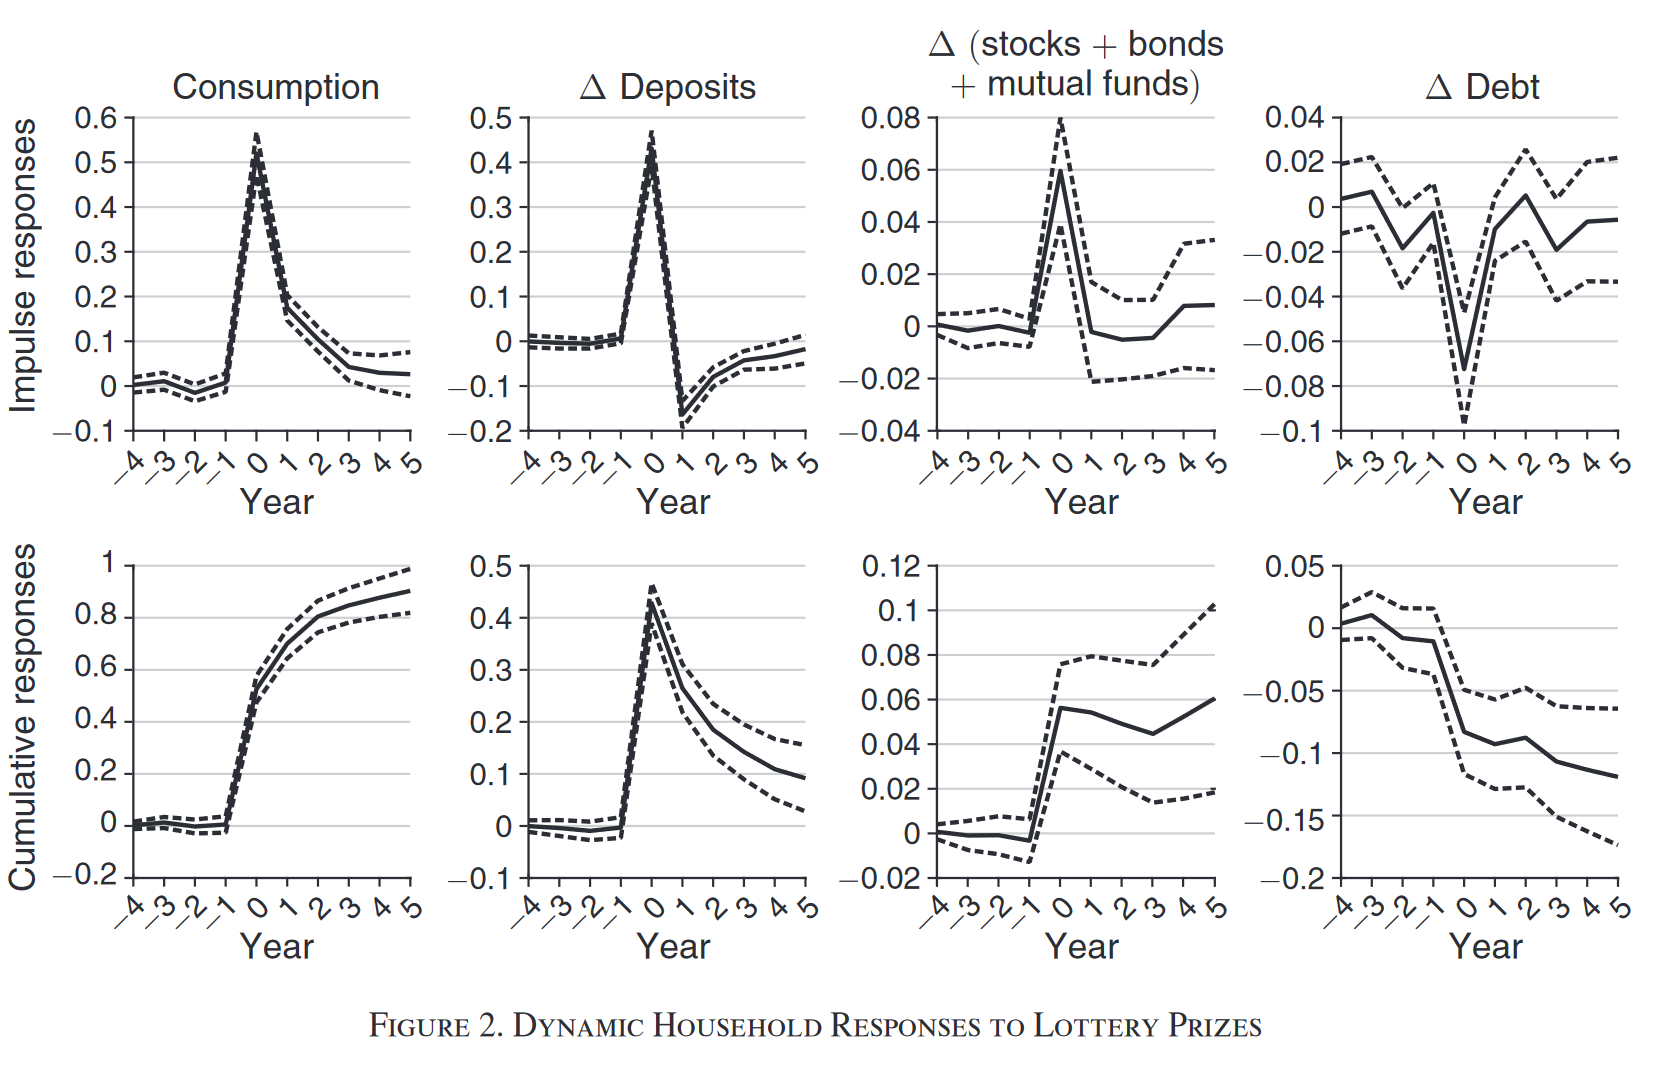
\includegraphics[width=1\textwidth]{figs/Fagereng_MPCs}

\textbf{Source:} Fagereng et. al. (2021)
\end{frame}
%
\begin{frame}{Initial liquidity/borrowing constraint}
\begin{itemize}
\item Implied period $0$ \textbf{savings} are\textbf{: $a_{0}=s_{0}+wz_{0}-c_{0}$}
\item Hard \textbf{borrowing constraint:} $a_{0}\geq-wb$
\item \textbf{Maximum consumption:} $\overline{c}_{0}=s_{0}+wz_{0}+wb$
\item \textbf{Optimal consumption: }Constrained or unconstrained.\texttt{
\[
c^{\ast}_{0}=\min\left\{ \overline{c}_{0},\left(1-\frac{(\beta R)^{1/\sigma}}{R}\right)(s_{0}+h_{0})\right\} 
\]
}
\item \textbf{Empirical realism.} MPC of constrained is one
\[
c^{\ast}_{0}=\overline{c}_{0}\Rightarrow\frac{\partial c^{\ast}_{0}}{\partial s_{0}}=\frac{\partial\overline{c}_{0}}{\partial s_{0}}=1
\]
\item \textbf{Technical issue: }\emph{Borrowing constraints further in the
future complicates the analytical solution considerably.}
\end{itemize}
\end{frame}
%

\section{Buffer-stock}
\begin{frame}{Uncertainty and always borrowing constraint}

\vspace{-8mm}
\begin{align*}
v_{0}(z_{0},a_{-1}) & =\max_{\{c_{t}\}^{\infty}_{t=0}}\mathbb{E}_{0}\left[\sum^{\infty}_{t=0}\beta^{t}u(c_{t})\right]\\
 & \text{s.t.}\\
a_{t} & =(1+r)a_{t-1}+wz_{t}-c_{t}\\
z_{t+1} & \sim\mathcal{Z}(z_{t})\\
a_{t} & \geq-wb\\
\lim_{t\rightarrow\infty}(1+r)^{-t}a_{t} & \geq0\,\,\,\,\,[\text{No-Ponzi game}]
\end{align*}

\begin{itemize}
\item \vspace{-3mm}\textbf{Stochastic income} from 1st order Markov-process,
$\mathcal{Z}$
\item \textbf{\emph{A true dynamic problem:}}
\begin{enumerate}
\item \textbf{Information: }$z_{t}$ is revealed period-by-period
\item \textbf{Target:} \emph{Expected} discounted utility, $\mathbb{E}_{0}\left[\sum^{\infty}_{t=0}\beta^{t}u(c_{t})\right]$
\item \textbf{Behavior: }Choose $c_{t}$ \emph{sequentially} as information
is revealed
\item \textbf{Solution:} Sequence of consumption \emph{functions}, $c^{\ast}_{t}(z_{t},a_{t-1})$
\end{enumerate}
\end{itemize}
\end{frame}
%
\begin{frame}{IBC}
\begin{itemize}
\item \textbf{Substitution }still implies:
\begin{eqnarray*}
R^{-(T-1)}a_{T-1}=0 & \Leftrightarrow & \sum^{\infty}_{t=0}R^{-t}c_{t}=s_{0}+h_{0}
\end{eqnarray*}
\item \textbf{What if $T\rightarrow\infty$? }We must have $\lim_{T\rightarrow\infty}R^{-(T-1)}a_{T-1}=0$
\begin{enumerate}
\item $\lim_{T\rightarrow\infty}R^{-(T-1)}a_{T-1}>0$: Consumption can be
increased
\item $\lim_{T\rightarrow\infty}R^{-(T-1)}a_{T-1}<0$: Violates No-Ponzi
game condition
\end{enumerate}
\item For $T\rightarrow\infty$ we have the\textbf{ IBC}:
\[
\sum^{\infty}_{t=0}R^{-t}c_{t}=Ra_{-1}+\sum^{\infty}_{t=0}R^{-t}wz_{t}
\]
\end{itemize}
\end{frame}
%
\begin{frame}{Natural borrowing limit}
\begin{itemize}
\item Denote \textbf{minimum possible productivity }by\textbf{ $\underline{z}$}
\item \textbf{Consumption must be non-negative} $\Rightarrow$\\
\emph{interest payments must be less than minimum income}
\[
c_{t}\geq0\Rightarrow r(-a_{t})\leq w\underline{z}\Leftrightarrow a_{t}\geq-\frac{w\underline{z}}{r}
\]
If debt was larger it would in the worst case ($\forall z_{t}=\underline{z}$)
grow without bound even with zero consumption ($\forall c_{t}=0$)
\begin{align*}
a_{0} & =-\frac{w\underline{z}}{r}-\Delta\\
a_{1} & =(1+r)a_{0}+w\underline{z}=a_{0}-(1+r)\Delta\\
a_{2} & =(1+r)a_{1}+w\underline{z}=a_{0}-(1+r)^{2}\Delta\\
\vdots
\end{align*}
\item \vspace{-2mm}\textbf{Natural borrowing constraint: $a_{t}\geq\underline{a}=-w\min\left\{ b,\frac{\underline{z}}{r}\right\} $}
\end{itemize}
\end{frame}
%
\begin{frame}{Euler-equation from variation argument}
\begin{itemize}
\item \textbf{Case I:} If $u^{\prime}(c_{t})>\beta R\mathbb{E}_{t}\left[u^{\prime}(c_{t+1})\right]$:

Increase $c_{t}$ by marginal $\Delta>0$, and lower $c_{t+1}$ by
$R\Delta$
\begin{enumerate}
\item \textbf{Feasible:} Yes, if $a_{t}>\underline{a}$
\item \textbf{Utility change: }For $\Delta\rightarrow0$ $u^{\prime}(c_{t})+\beta\left(-R\right)\mathbb{E}_{t}\left[u^{\prime}(c_{t+1})\right]>0$\vspace{2mm}
\end{enumerate}
\item \textbf{Case II:} If $u^{\prime}(c_{t})<\beta R\mathbb{E}_{t}\left[u^{\prime}(c_{t+1})\right]$: 

Lower $c_{t}$ by marginal $\Delta>0$, and increase $c_{t+1}$ by
$R\Delta$
\begin{enumerate}
\item \textbf{Feasible:} Yes (always)
\item \textbf{Utility change: }For $\Delta\rightarrow0$\textbf{ }$u^{\prime}(c_{t})+\beta R\mathbb{E}_{t}\left[u^{\prime}(c_{t+1})\right]>0$\vspace{2mm}
\end{enumerate}
\item \textbf{Conclusion: }By contradiction
\begin{enumerate}
\item \textbf{Constrained:} $a_{t}=\underline{a}$ and $u^{\prime}(c_{t})\geq\beta R\mathbb{E}_{t}\left[u^{\prime}(c_{t+1})\right]$,
or
\item \textbf{Unconstrained:} $a_{t}>\underline{a}$ and $u^{\prime}(c_{t})=\beta R\mathbb{E}_{t}\left[u^{\prime}(c_{t+1})\right]$
\end{enumerate}
\item \textbf{Sufficiency: }Harder ($\sim$ convexity of the choice set)
\end{itemize}
\end{frame}
%
\begin{frame}{Special case I: Quadratic utility}
\begin{itemize}
\item \textbf{Quadratic utility:} $u(c_{t})=-\frac{1}{2}(\overline{c}-c)^{2}$
with $\beta R=1$ and >>large<< $\overline{c}$ 
\item \textbf{Euler-equation: }\emph{Consumption = expected future consumption}
\begin{align*}
(\overline{c}-c_{t}) & =\mathbb{E}_{t}\left[(\overline{c}-c_{t+k})\right]\Leftrightarrow c_{t}=\mathbb{E}_{t}\left[c_{t+k}\right]
\end{align*}
\item Use \textbf{IBC }in expectation\textbf{ }to get \textbf{consumption
function:}
\begin{align*}
\sum^{\text{\ensuremath{\infty}}}_{t=0}R^{-t}\mathbb{E}_{0}\left[c_{t}\right] & =Ra_{-1}+\sum^{\text{\ensuremath{\infty}}}_{t=0}R^{-t}w\mathbb{E}_{0}\left[z_{t}\right]\Rightarrow\\
c^{\ast}(z_{t},a_{t-1})=c_{0} & =ra_{-1}+\frac{r}{R}\sum^{T}_{t=0}R^{-t}w\mathbb{E}_{0}\left[z_{t}\right]
\end{align*}
where we formally disregard the borrowing constraint
\item \textbf{Certainty equivalence:} \emph{Only expected income matter}.
\end{itemize}
\end{frame}
%
\begin{frame}{Special case II: CARA utility}
\begin{itemize}
\item \textbf{CARA utility:} $u(c_{t})=-\frac{1}{\alpha}e^{-\alpha c}$
\item \textbf{Productivity is absolute random walk:}
\begin{align*}
z_{t} & =z_{t-1}+\psi_{t}\\
\psi_{t} & \sim\mathcal{N}(0,\sigma^{2}_{\psi})
\end{align*}
\item \textbf{Consumption function }({\color{DarkRed}\href{https://www.econ2.jhu.edu/people/ccarroll/public/LectureNotes/Consumption/CARAModelWithYRisk/}{see proof}})\textbf{:}
\[
c^{*}(a_{t-1},z_{t})=ra_{t-1}+wz_{t}-\frac{\log\left(\beta R\right)^{\frac{1}{\alpha}}+\alpha\frac{\sigma^{2}_{\psi}}{2}}{r^{2}}
\]
where we formally disregard the borrowing constraint
\item \textbf{Precautionary saving: }$\sigma^{2}_{\psi}\uparrow$ implies
$c^{*}_{t}\downarrow$ for given $z_{t}$ and $a_{t-1}$

$\Rightarrow$ \emph{accumulation of buffer-stock} 
\end{itemize}
\end{frame}
%
\begin{frame}{Dynamic solution: Bellman's Principle of Optimality}
\begin{itemize}
\item Go back to a \textbf{finite horizon} problem with $T$ periods
\item \textbf{Value function, $v_{t}$:} Defined \emph{recursively} from
$v_{T}(\bullet)=0$ 
\begin{align*}
v_{t}(z_{t},a_{t-1}) & =\max_{c_{t}}u(c_{t})+\beta\mathbb{E}_{t}[v_{t+1}(z_{t+1},a_{t})]\\
 & \text{s.t. }a_{t}=(1+r)a_{t-1}+wz_{t}-c_{t}\geq\underline{a}
\end{align*}
\item \textbf{Policy function, $c^{*}_{t}$: }Is the same as
\begin{align*}
c^{*}_{t}(z_{t},a_{t-1}) & =\arg\max_{c_{t}}u(c_{t})+\beta\mathbb{E}_{t}[v_{t+1}(z_{t+1},a_{t})]\\
 & \text{s.t. }a_{t}=(1+r)a_{t-1}+wz_{t}-c_{t}\geq\underline{a}
\end{align*}
\item \textbf{Euler-equation:}
\begin{enumerate}
\item FOC: $c^{-\sigma}_{t}=\beta\mathbb{E}_{t}\left[v_{t,a}(z_{t+1},a_{t})\right]$
\item Envelope: $v_{t,a}(z_{t},a_{t-1})=(1+r)c^{-\sigma}_{t}$ (fix $a_{t}$)
\end{enumerate}
\end{itemize}
\end{frame}
%
\begin{frame}{Vocabulary}

\vspace{-7mm}
\begin{align*}
v_{t}(z_{t},a_{t-1}) & =\max_{c_{t}}u(c_{t})+\beta\mathbb{E}_{t}[v_{t+1}(z_{t+1},a_{t})]\\
 & \text{s.t. }a_{t}=(1+r)a_{t-1}+wz_{t}-c_{t}\geq\underline{a}
\end{align*}

\begin{enumerate}
\item \vspace{-3mm}\textbf{State variables: }$z_{t}$ and $a_{t-1}$
\item \textbf{Control }(choice)\textbf{ variable:} $c_{t}$
\item \textbf{Continuation value:} $\beta\mathbb{E}_{t}[v_{t+1}(z_{t+1},a_{t})]$
\item \textbf{Parameters: }$r$, $w$, and stuff in $u(\bullet)$
\end{enumerate}
\textbf{Note:} Straightforward to extend to more goods, more assets
or other states, more complex risk, bounded rationality etc. 
\end{frame}
%
\begin{frame}{Infinite horizon: $T\rightarrow\infty$}

\vspace{-7mm}
\begin{align*}
v_{t}(z_{t},a_{t-1}) & =\max_{c_{t}}u(c_{t})+\beta\mathbb{E}_{t}[v_{t+1}(z_{t+1},a_{t})]\\
 & \text{s.t. }a_{t}=(1+r)a_{t-1}+wz_{t}-c_{t}\geq\underline{a}
\end{align*}

\begin{itemize}
\item \vspace{-3mm}\textbf{Contraction mapping result:} \emph{If $\beta$
is low enough (strong enough impatience) then the value and policy
functions converge to $v(z_{t},a_{t-1})$ and $c^{\ast}(z_{t},a_{t-1})$
for large enough $T$}
\item \textbf{In practice:} 
\begin{enumerate}
\item Make arbitrary initial guess (e.g. $v_{T}=0$)
\item Solve backwards until the value (and/or policy function) does not
change anymore (relative to chosen tolerance)
\end{enumerate}
\end{itemize}
\end{frame}
%

\section{3-periods}
\begin{frame}{3-period model}
\begin{itemize}
\item \textbf{Expected discounted utility:} $v(z_{0},a_{-1})=\mathbb{E}_{0}\sum^{2}_{t=0}\beta^{t}\frac{c^{1-\sigma}_{t}}{1-\sigma}$
\item \textbf{Income $=$ wage $\times$ productivity + transfer:}
\[
y_{t}=wz_{t}+\chi_{t}
\]
\item \textbf{Cash-on-hand, savings and borrowing constraint:}
\begin{align*}
m_{t} & =(1+r)a_{t-1}+y_{t}\\
a_{t} & =m_{t}-c_{t}\\
a_{t} & \geq\underline{a}
\end{align*}
\item \textbf{Stochastic transition: }$\text{Pr}\left[z_{t+1}|z_{t}\right]=\pi_{t}(z_{t},z_{t+1})$
such that
\begin{align*}
\text{Pr}\left[z_{t+1}=1\,|\,z_{t}=1\right] & =\pi\\
\text{Pr}\left[z_{t+1}=1-\Delta\,|\,z_{t}=1\right]=\text{Pr}\left[z_{t+1}=1+\Delta\,|\,z_{t}=1\right] & =\frac{1-\pi}{2}\\
\text{Pr}\left[z_{t+1}=z_{t}\,|\,z_{t}\in\{1-\Delta,1+\Delta\}\right] & =1
\end{align*}
\end{itemize}
\end{frame}
%
\begin{frame}{Bellman equation}

\vspace{-6mm}
\begin{align*}
v_{t}(z_{t},a_{t-1}) & =\max_{c_{t}}\frac{c^{1-\sigma}_{t}}{1-\sigma}+\beta\mathbb{E}_{t}\left[v_{t+1}(z_{t+1},a_{t})\right]\\
 & \text{s.t.}\\
y_{t} & =wz_{t}+\chi_{t}\\
m_{t} & =(1+r)a_{t-1}+y_{t}\\
a_{t} & =m_{t}-c_{t}\\
\text{Pr}\left[z_{t+1}|z_{t}\right] & =\pi_{t}(z_{t},z_{t+1})\\
a_{t} & \geq\underline{a}
\end{align*}
where 
\[
v_{3}(z_{3},a_{2})=0
\]

\end{frame}
%
\begin{frame}[fragile]{Discretization}
\begin{itemize}
\item \textbf{Discretization: }All state variables belong to discrete sets
$\equiv$ \emph{grids},\vspace{-2mm}
\begin{align*}
z_{t} & \in\mathcal{G}_{z}=\{z^{0},z^{1},\dots,z^{\#z-1}\}\\
a_{t} & \in\mathcal{G}_{a}=\{a^{0},a^{1},\dots,a^{\#_{a}-1}\}\\
 & a^{0}=\underline{a}
\end{align*}
\item \textbf{Expectation: }Numerical integration by\textbf{
\begin{align*}
\mathbb{E}_{t}\left[v_{t+1}(z_{t+1},a_{t})\right] & =\sum_{z_{t+1}\in\left\{ 1-\Delta,1,1+\Delta\right\} }\pi_{t}(z_{t},z_{t+1})v_{t+1}(z_{t+1},a_{t})
\end{align*}
}
\item \textbf{ConSav: }\lstinline{grids.nonlinspace}, \lstinline{grids.equilogspace}
\item \textbf{ConSavNotebooks: }\lstinline{04. Tools/03. Grids.ipynb} 
\end{itemize}
\end{frame}
%
\begin{frame}{Grids and transition probabilities}

\begin{tabular}{cc}

\includegraphics[width=0.57\textwidth]{01_ConSavModel_3periods/figs/grids} & 
\includegraphics[width=0.43\textwidth]{01_ConSavModel_3periods/figs/z_trans}\tabularnewline
\end{tabular}

The size of risk is scaled by $\Delta$

Baseline: $\Delta=0.8$

Low risk: $\Delta=0.4$
\end{frame}
%
\begin{frame}[fragile]{Linear interpolation}
\begin{itemize}
\item \textbf{Linear interpolation }(function approximation):\vspace{1mm} 
\begin{enumerate}
\item Assume $v_{t+1}$ is known on $\mathcal{G}_{z}\times\mathcal{G}_{a}$
(tensor product)
\item Evaluate $v_{t+1}(z^{i_{z}},a)$ for arbitrary $a$ by\vspace{-2mm}
\begin{align*}
\breve{v}_{t+1}(z^{i_{z}},a) & =\text{baseline + slope}\times\text{distance}\\
 & =v_{t+1}(z^{i_{z}},a^{\iota})+\omega(a-a^{\iota})\\
 & \text{where}\\
 & \omega\equiv\frac{v_{t+1}(z^{i_{z}},a^{\iota+1})-v_{t+1}(z^{i_{z}},a^{\iota})}{a^{\iota+1}-a^{\iota}}\\
 & \iota\equiv\text{largest }i_{a}\in\{0,1,\dots,\#_{a}-2\}\text{ such that }a^{i_{a}}\leq a
\end{align*}
\end{enumerate}
\item \textbf{ConSav: }\lstinline{linear_interp.interp1d} 
\item \textbf{ConSavNotebooks: }\lstinline{04. Tools/01. Linear interpolation.ipynb} 
\end{itemize}
\end{frame}
%
\begin{frame}{Linear interpolation}


\includegraphics[width=0.95\textwidth]{01_ConSavModel_3periods/figs/linear_interpolation}
\end{frame}
%
\begin{frame}[fragile]{Value function iteration (VFI)}
\begin{itemize}
\item \textbf{Maximize value-of-choice:}
\begin{align*}
v_{t}(z^{i_{z}},a^{i_{a-}}) & =\max_{c_{t}}v_{t}(z^{i_{z}},a^{i_{a-}}|c_{t})\\
 & \text{with }c_{t}\in[0,(1+r)a^{i_{a-}}+wz^{i_{z}}+\chi_{t}+\underline{a}]
\end{align*}
\vspace{-7mm}
\begin{align*}
v_{t}(z^{i_{z}},a^{i_{a-}}|c_{t}) & =u(c_{t})+\beta\sum^{\#_{z}-1}_{i_{z+1}=0}\pi\left(i_{z},i_{z+1}\right)\breve{v}_{t+1}(z^{i_{z}},a_{t})\\
 & \text{with }a_{t}=(1+r)a^{i_{a-}}+wz^{i_{z}}+\chi_{t}-c_{t}
\end{align*}
\item \textbf{Inner loop: }For each grid point in $\mathcal{G}_{z}\times\mathcal{G}_{a}$
find $c^{\ast}_{t}(z_{t},a_{t-1})$ and therefore $v_{t}(z_{t},a_{t-1})$
with a \emph{numerical optimizer}
\item \textbf{Outer loop: }Backwards from $t=T-1$ (note $\underline{v}_{T}=0$,
or known)
\item \textbf{ConSav+QuantEcon: }Various optimizers in \lstinline{numba} 
\item \textbf{ConSavNotebooks: }\lstinline{04. Tools/02. Optimization.ipynb} 
\end{itemize}
\end{frame}
%
\begin{frame}{Consumption function}


\includegraphics[width=0.95\textwidth]{01_ConSavModel_3periods/figs/c_func}
\end{frame}
%
\begin{frame}{Savings function}


\includegraphics[width=0.95\textwidth]{01_ConSavModel_3periods/figs/a_func}
\end{frame}
%
\begin{frame}{Change in savings function}


\includegraphics[width=0.95\textwidth]{01_ConSavModel_3periods/figs/a_diff_func}
\end{frame}
%
\begin{frame}{MPC}


\includegraphics[width=0.95\textwidth]{01_ConSavModel_3periods/figs/MPC}
\end{frame}
%
\begin{frame}{Intertemporal MPC}

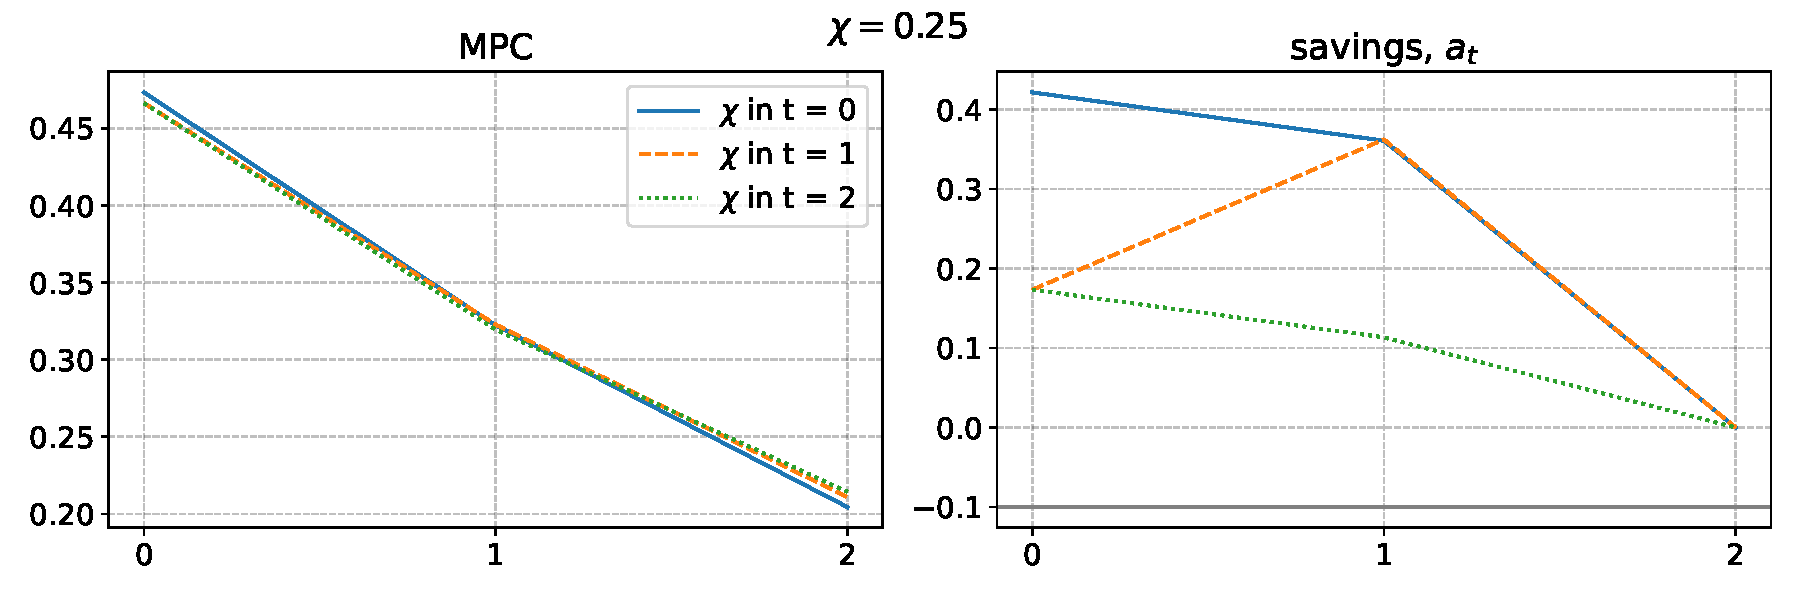
\includegraphics[width=0.95\textwidth]{01_ConSavModel_3periods/figs/MPC_dyn_1}

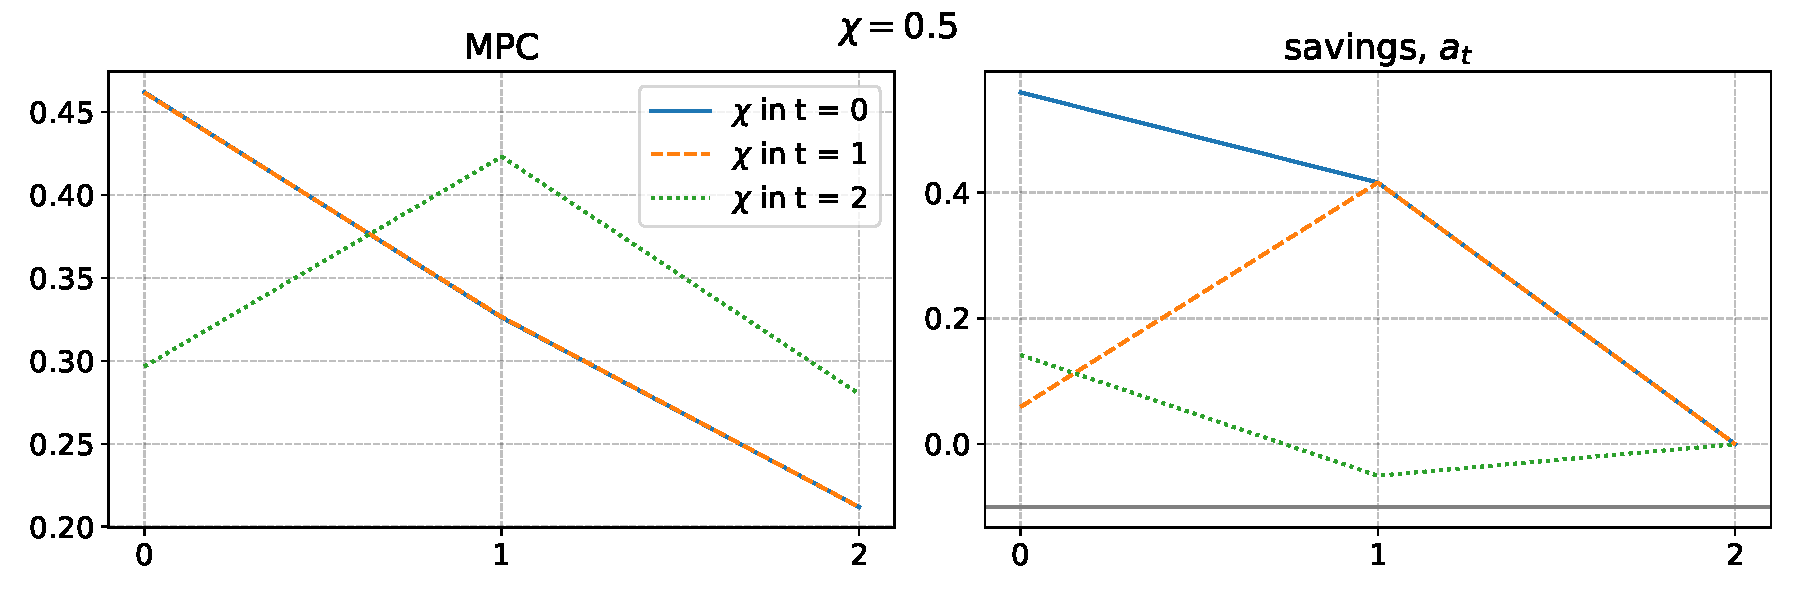
\includegraphics[width=0.9\textwidth]{01_ConSavModel_3periods/figs/MPC_dyn_2}

Note: No wealth effect as $r=0$
\end{frame}
%
\begin{frame}{Economic insights}
\begin{itemize}
\item \textbf{Notebook: }01\_ConSavModel\_3periods/ConSavModel.ipynb
\item \textbf{Consumption lower than under PIH and concave in assets}

\textbf{Intuition:} \emph{Precautionary saving motive is relatively
larger for asset poor households because income risk is the same for
everybody}

\textbf{Implications:}
\begin{enumerate}
\item Windfall gives safety and increases average consumption \\
$\Rightarrow$ MPC decreasing in assets
\item Attraction towards a buffer-stock target $a_{t}=a_{t-1}$ despite
$\beta R<1$
\item Larger effective discounting of future income

(extreme: no effect of future income changes if constrained before)
\end{enumerate}
\end{itemize}
\end{frame}
%
\begin{frame}{Numerical Monte Carlo simulation}
\begin{itemize}
\item \textbf{Initial distribution: }Draw $z_{i,-1}$ and $a_{i,-1}$ for
$i\in\{0,1,\dots,N-1\}$ 
\item \textbf{Simulation: }Forwards in time from $t=0$ and in each time
period
\begin{enumerate}
\item Draw $z_{it}$ given transition probabilities
\item Use linear interpolation to evaluate\vspace{-1mm} 
\begin{align*}
c_{it} & =\breve{c}^{\ast}_{t}(z_{it},a_{it-1})\\
a_{it} & =(1+r)a_{it-1}+wz_{it}-c_{it}
\end{align*}
\end{enumerate}
\item \textbf{Review:}
\begin{itemize}
\item \textbf{Pro:} Simple to implement
\item \textbf{Con:} Computationally costly and introduces randomness
\end{itemize}
\item \textbf{Infinite horizon: }
\begin{enumerate}
\item Assume $z_{it}$ has an ergodic distribution
\item Ergodic distribution of $a_{it}$ around buffer-stock target 
\end{enumerate}
\end{itemize}
\end{frame}
%
\begin{frame}{Taking stock}
\begin{itemize}
\item \textbf{Value Function Iteration (VFI)}
\begin{enumerate}
\item Solve all consumption-saving models
\item Accurate with dense enough grids
\item Relatively simple code and easy to run in parallel
\item Finding optimal choices is the computational bottleneck\\
(especially with multi-starts in non-convex models)
\end{enumerate}
\end{itemize}
\end{frame}

\section{EGM}
\begin{frame}{Time iteration}
\begin{itemize}
\item \textbf{Replace numerical optimization with root-finding}
\item \textbf{Time iteration:} For each $a_{t-1}$ and $z_{t}$ find $c_{t}$
to solve the Euler-equation
\[
c^{-\sigma}_{t}=\beta(1+r)\mathbb{E}_{t}[c^{-\sigma}_{t+1}]
\]

Note: \emph{Necessary and sufficient} (for interior choices, else
$a_{t}=\underline{a}$)
\item \textbf{EGM:} No need for any numerical optimization or root-finding
\end{itemize}
\end{frame}
%
\begin{frame}{Endogenous grid-point method (EGM)}
\begin{enumerate}
\item Calculate\textbf{ post-decision marginal value of cash:}\vspace{-1mm}
\[
q(z^{i_{z}},a^{i_{a}})=\sum^{\#_{z}-1}_{i_{z+}=0}\pi_{i_{z},i_{z+}}c^{\ast}_{+}(z^{i_{z+}},a^{i_{a}})^{-\sigma}
\]
\item \vspace{-2mm}\textbf{Invert Euler-equation:}\vspace{-1mm}
\[
c(z^{i_{z}},a^{i_{a}})=(\beta(1+r)q(z^{i_{z}},a^{i_{a}}))^{-\frac{1}{\sigma}}
\]
\item \vspace{-1mm}\textbf{Endogenous cash-on-hand:}\vspace{-1mm}
\[
m(z^{i_{z}},a^{i_{a}})=a^{i_{a}}+c(z^{i_{z}},a^{i_{a}})
\]
\item \vspace{-1mm}\textbf{Consumption function:} Calculate $m=(1+r)a^{i_{a-}}+wz^{i_{z}}$\vspace{1mm}
\begin{enumerate}
\item Binding constraint: If $m\leq m(z^{i_{z}},a^{0})$ then\vspace{-1mm}
\[
c^{\ast}(z^{i_{z}},a^{i_{a-}})=m+\underline{a}
\]
\item \vspace{-3mm}Interior choice: Else\vspace{-1mm}
\[
c^{\ast}(z^{i_{z}},a^{i_{a-}})=\text{interpolate }m(z^{i_{z}},m)\rightarrow c(z^{i_{z}},m)
\]
\end{enumerate}
\end{enumerate}
\end{frame}
%

\section{Income process}
\begin{frame}[fragile]{Permanent transitory income process}
\begin{itemize}
\item \textbf{Persistent-transitory income process: }
\begin{align*}
z_{t} & =\tilde{z}_{t}\xi_{t},\,\,\,\log\xi_{t}\sim\mathcal{N}(\mu_{\xi},\sigma_{\xi})\\
\log\tilde{z}_{t+1} & =\rho_{z}\log\tilde{z}_{t}+\psi_{t+1},\,\,\,\psi_{t+1}\sim\mathcal{N}(\mu_{\psi},\sigma_{\psi})
\end{align*}

\begin{enumerate}
\item Transitory shock: $\xi_{t}$
\item Persistent shock: $\psi_{t}$
\item Normalization using $\mu_{\psi}$ and $\mu_{\xi}$: $\mathbb{E}\left[z_{t}\right]=\mathbb{E}\left[\tilde{z}_{t}\right]=1$
\end{enumerate}
\item \textbf{ConSav: }\lstinline{qudarature.log_normal_gauss_hermite} 
\item \textbf{ConSavNotebook: }\lstinline{04. Tools/04. Quadrature.ipynb} 
\end{itemize}
\end{frame}
%
\begin{frame}[fragile]{Transition probabilities}
\begin{itemize}
\item \textbf{Discretization of $\xi_{t}$: }Derive $\mathcal{G}_{\xi}$
and $\pi_{i_{\xi}}$ given $\sigma_{\xi}$ using Gauss-Hermite quadrature
\[
x\sim\mathcal{N}(\mu,\sigma^{2}):\,\,\,\mathbb{E}[h(x)]\approx\frac{1}{\sqrt{\pi}}\sum^{n}_{i=1}\omega_{i}h(\sqrt{2}\sigma x_{i}+\mu)
\]
where nodes, $x_{i}$, and weights, $\omega_{i}$, have analytical
expressions
\item \textbf{Discretization of $\tilde{z}_{t}$: }Derive\textbf{ }$\mathcal{G}_{\tilde{z}}$
and $\pi_{i_{\tilde{z}-},i_{\tilde{z}}}$ given $\rho_{z}<1$ and
$\sigma_{\psi}$ (using a method such as Tauchen (1986) or Rouwenhorst
(1995))

If $\rho_{z}=1$: Also use quadrature here.
\item \textbf{Combined:} Derive $\mathcal{G}_{z}=\mathcal{G}_{\tilde{z}}\times\mathcal{G_{\xi}}$
(tensor product) and use independence of $\tilde{z}_{t}$ and $\xi_{t}$
to get transition probabilities $\pi_{i_{z-},i_{z}}$ (kronecker product)
\item \textbf{ConSav: }\lstinline{markov.log_rouwenhorst}, \lstinline{markov.log_tauchen}
\item \textbf{ConSavNotebook: }\lstinline{04. Tools/05. Markov.ipynb}
\end{itemize}
\end{frame}
%

\section{Full household problem}
\begin{frame}{Full household problem}
\begin{itemize}
\item \textbf{Utility maximization} for household $i$:\vspace{-2mm}
\begin{align*}
v_{0}(z_{t},a_{t-1}) & =\max_{\{c_{t}\}^{\infty}_{t=0}}\mathbb{E}_{0}\sum^{\infty}_{t=0}\beta^{t}u(c_{t})\\
 & \text{s.t.}\\
a_{t} & =(1+r_{t})a_{t-1}+wz_{t}-c_{it}\\
\log z_{t+1} & =\rho_{z}\log z_{t}+\psi_{t+1},\,\,\,\psi_{t}\sim\mathcal{N}(\mu_{\psi},\sigma_{\psi}),\,\,\,\mathbb{E}[z_{t}]=1\\
a_{t} & \geq-bw
\end{align*}
\end{itemize}
\end{frame}
%
\begin{frame}{Recursive formulation I}
\begin{itemize}
\item \textbf{Value function}:
\begin{align*}
v(z_{t},a_{t-1}) & =\max_{c_{t}}u(c_{t})+\beta\mathbb{E}_{t}\left[v(z_{t+1},a_{t})\right]\\
 & \text{s.t.}\\
a_{t} & =(1+r)a_{t-1}+wz_{t}-c_{t}\\
\log z_{t+1} & =\rho_{z}\log z_{t}+\psi_{t+1}\\
a_{t} & \geq-bw
\end{align*}
\item \textbf{Same Euler-equation}
\item \textbf{Borrowing constrained }has
\begin{align*}
c_{it} & =m_{it}-bw
\end{align*}
where $m_{t}=(1+r)a_{t-1}+wz_{t}$
\end{itemize}
\end{frame}
%
\begin{frame}{Recursive formulation II}
\begin{itemize}
\item \textbf{Beginning-of-period value function
\[
\underline{v}\left(z_{t-1},a_{t-1}\right)=\mathbb{E}\left[v(z_{t},a_{t-1})\,|\,z_{t-1}\right]
\]
}
\item \textbf{Value function}:
\begin{align*}
v(z_{t},a_{t-1}) & =\max_{c_{t}}u(c_{t})+\beta\underline{v}\left(z_{t},a_{t}\right)\\
 & \text{s.t.}\\
a_{t} & =(1+r)a_{t-1}+wz_{t}-c_{t}\\
\log z_{t+1} & =\rho_{z}\log z_{t}+\psi_{t+1}\\
a_{t} & \geq-bw
\end{align*}
\item \textbf{Why do this? }\emph{Only one interpolation per guess of $c_{t}$}
\end{itemize}
\end{frame}
%
\begin{frame}{Distribution}
\begin{itemize}
\item \textbf{Problem with Monte Carlo simulation:} \emph{Stochastic fluctuations
in average wealth $\text{\ensuremath{\Rightarrow} }$stochastic error
in asset market clearing condition.}
\item \textbf{Alternative – Histogram:} Distribution as array of probabilities
\begin{enumerate}
\item Beginning-of-period: $\underline{\boldsymbol{D}}_{t}$ over $z_{it-1}$
and $a_{it-1}$\vspace{1mm}
\item Productivity transition: $\boldsymbol{D}_{t}=\Pi^{\prime}_{z}\underline{\boldsymbol{D}}_{t}$
over $z_{it}$ and $a_{it-1}$\vspace{1mm}
\item Savings transition: $\underline{\boldsymbol{D}}_{t+1}=\Lambda^{\prime}\boldsymbol{D}_{t}$
where $\Lambda$ derives from $a^{\ast}(z_{t},a_{t-1})$\vspace{-1mm}
\end{enumerate}
\end{itemize}
\end{frame}
%
\begin{frame}{Numerical histogram simulation}
\begin{itemize}
\item <+->\textbf{Initial distribution: }Choose $\underline{\boldsymbol{D}}_{0}(z_{-1},a_{-1})$,
which is defined on $\mathcal{G}_{z}\times\mathcal{G}_{a}$ and sum
to $1$ $\equiv$ \emph{histogram}
\item <+->\textbf{Simulation: }Forwards in time from $t=0$ and in each
time period
\begin{enumerate}
\item <+->\textbf{Distribute stochastic mass:} For each $i_{z}$ and $i_{a-}$
calculate\vspace{-2mm}

\[
\boldsymbol{D}_{t}(z^{i_{z}},a^{i_{a-}})=\sum^{\text{\#}_{z}-1}_{i_{z-}=0}\pi_{i_{z-},i_{z}}\boldsymbol{\underline{\boldsymbol{D}}}_{t}(z^{i_{z-}},a^{i_{a-}})
\]

\item <+->\textbf{Initial zero mass:} Set $\underline{\boldsymbol{D}}_{t+1}(z^{i_{z}},a^{i_{a}})=0$
for all $i_{z}$ and $i_{a}$\vspace{2mm}
\item <+->\textbf{Distribute endogenous mass:} For each $i_{z}$ and $i_{a-}$
do\vspace{2mm}
\begin{enumerate}
\item <+->Find $\iota\equiv\text{largest }i_{a}\in\{0,1,\dots,\#_{a}-2\}$
such that $a^{i_{a}}\leq a^{\ast}(z^{i_{z}},a^{i_{a-}})$\vspace{2mm}
\item <+->Calculate $\omega=\frac{a^{\iota+1}-a^{\ast}(z^{i_{z}},a^{i_{a-}})}{a^{\iota+1}-a^{\iota}}\in[0,1]$\vspace{2mm}
\item <+->Increment $\underline{\boldsymbol{D}}_{t+1}(z^{i_{z}},a^{\iota})$
with $\omega\boldsymbol{D}_{t}(z^{i_{z}},a^{i_{a-}})$\vspace{2mm}
\item <+->Increment $\boldsymbol{\underline{\boldsymbol{D}}}_{t+1}(z^{i_{z}},a^{\iota+1})$
with $(1-\omega)\boldsymbol{D}_{t}(z^{i_{z}},a^{i_{a-}})$
\end{enumerate}
\end{enumerate}
\end{itemize}
\end{frame}
%
\begin{frame}{Implementation}
\begin{itemize}
\item <+->\textbf{Toy example: }simple\_histogram\_simulation.xlsx\vspace{1mm}
\begin{itemize}
\item \textbf{Grids:} $\mathcal{G}_{z}=\{\underline{z},\overline{z}\}$
and $\mathcal{G}_{a}=\{0,1\}$\vspace{1mm}
\item \textbf{Transition matrix:} $\pi_{0,0}=\pi_{1,1}=0.5$\vspace{1mm}
\item \textbf{Policy function: }
\begin{itemize}
\item Low income: $a^{\ast}(\underline{z},0)=a^{\ast}(\underline{z},1)=0$
\item High income: Let $a^{\ast}(\overline{z},0)=0.5$ and $a^{\ast}(\overline{z},1)=1$\vspace{1mm}
\end{itemize}
\item \textbf{Initial distribution}: $\underline{\boldsymbol{D}}_{0}(z_{it},a_{it-1})=\begin{cases}
1 & \text{if }z_{it}=\underline{z}\text{ and }a_{it}=0\\
0 & \text{else}
\end{cases}$\vspace{1mm}
\item \textbf{Task: }Calculate by hand the transitions to
\[
\boldsymbol{D}_{0},\,\underline{\boldsymbol{D}}_{1},\,\boldsymbol{D}_{1},\dots
\]
\end{itemize}
\item <+->\textbf{Comparison with Monte Carlo:} See 02\_ConSavModel\_infConSavModel/
\begin{enumerate}
\item \textbf{Pro: }Computationally efficient and no randomness
\item \textbf{Con: }Introduces a non-continuous distribution\vspace{2mm}
\end{enumerate}
\end{itemize}
\end{frame}
%

\section{Misc}
\begin{frame}{1. Life-cycle (I)}
\begin{itemize}
\item \textbf{Basically:}
\begin{enumerate}
\item Born, working, retied, die
\item Age-varying parameters (esp. income)
\end{enumerate}
\item \textbf{Add-ons:}
\begin{enumerate}
\item Labor supply, human capital, occupation
\item Portfolio choice and entrepreneurship
\item Family formation
\item Health, mortality
\item []etc.
\end{enumerate}
\item \textbf{Good starting example:} >>Life‐Cycle Consumption and Children:
Evidence from a Structural Estimation<<, Jørgensen (2017)
\end{itemize}
\end{frame}
%
\begin{frame}{1. Life-cycle (II)}

\vspace{-2mm}
\begin{columns}[T] % align columns
\begin{column}{.55\textwidth}

\textbf{Paper:} Gourinchas and Parker (2021)

\emph{Life-cycle consumption-saving model with retirement}
\begin{itemize}
\item Young households: \\
Save for precautionary reasons (buffer)
\item Older households:\\
Save for retirement (life-cycle)
\end{itemize}
\end{column}

\begin{column}{.55\textwidth}

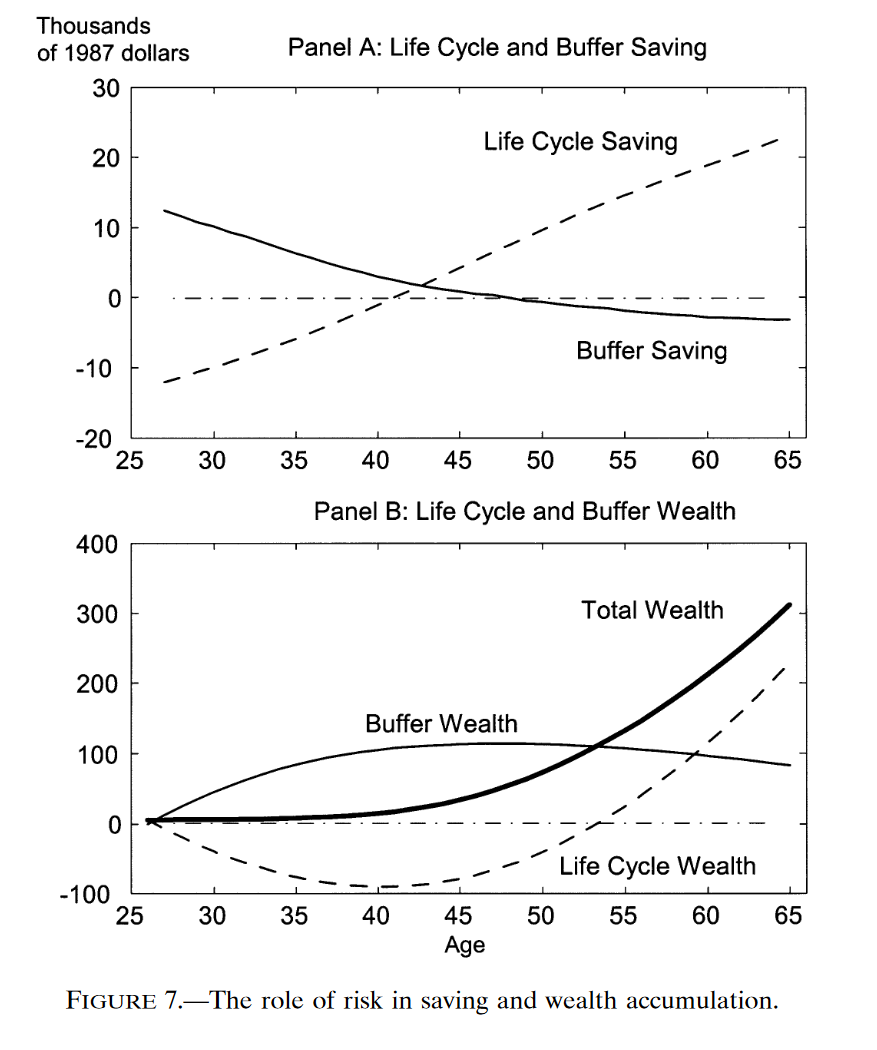
\includegraphics[width=1\textwidth]{figs/GourchasParker}

\end{column}

\end{columns}
\end{frame}
%
\begin{frame}{1 Life-cycle (III)}
\begin{itemize}
\item \textbf{Natural experiment:} Wealth depletion after sudden inheritance
\item \textbf{Results:}
\begin{enumerate}
\item Life-cycle profile of wealth fitted for many levels of risk-aversion\\
(by varying the discount factor)
\item Fast wealth depletation requires high risk-aversion\\
(or high perceived risk)
\end{enumerate}
\end{itemize}
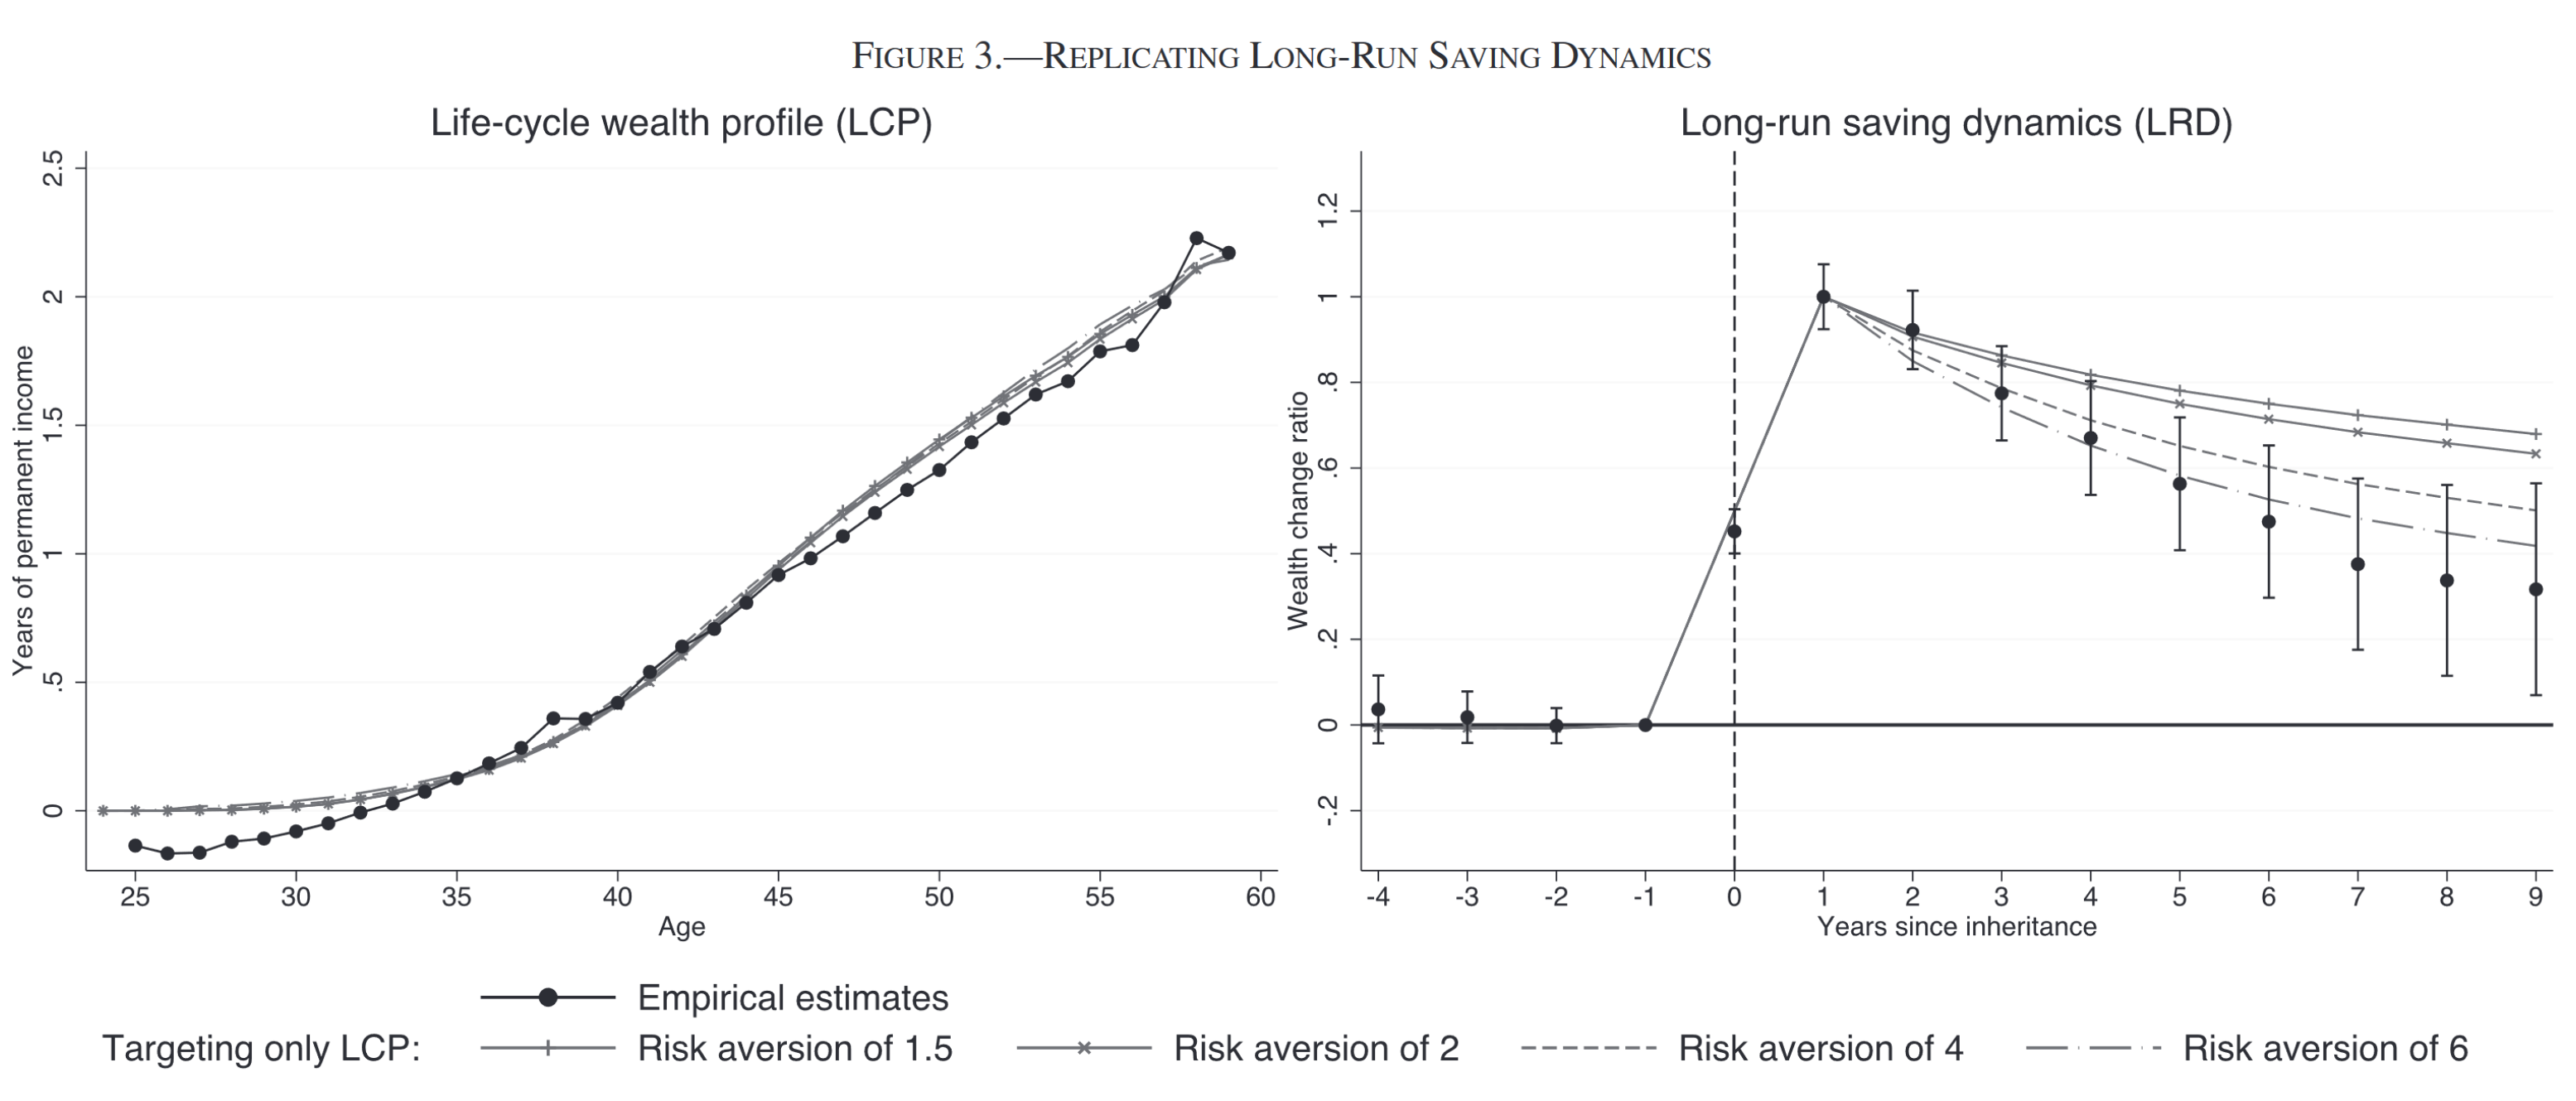
\includegraphics[width=0.95\textwidth]{figs/Druedahl_Martinello}\\
Source: Druedahl and Martinello (2022)
\end{frame}
%
\begin{frame}{2. More realistic income risk (I)}

Annual earnings-changes are far from log-normal:

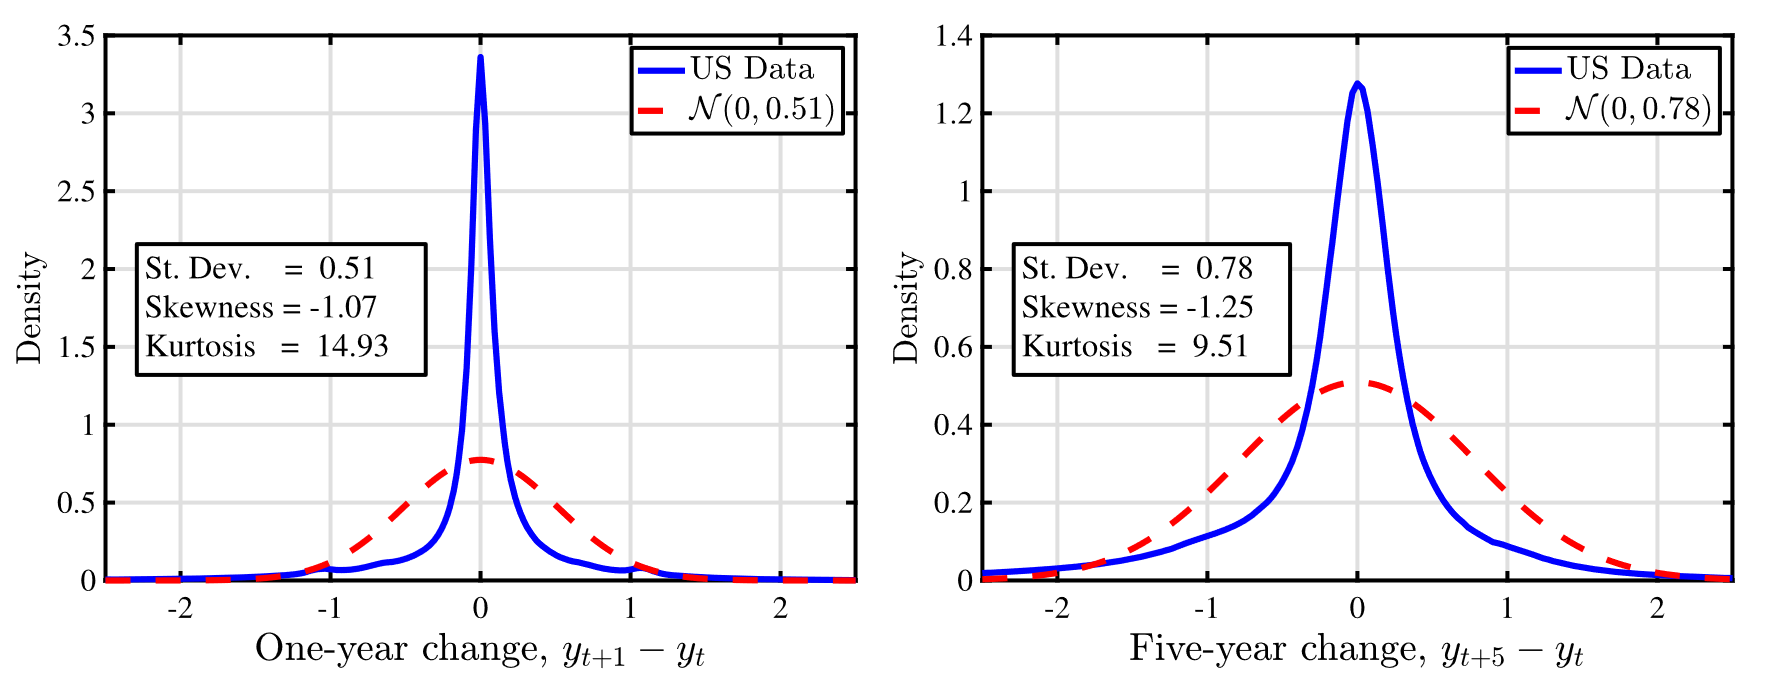
\includegraphics[width=1\textwidth]{figs/Guvenen}

Source: Guvenen et. al. (2021)
\end{frame}
%
\begin{frame}{2. More realistic income risk (II)}

Many with zero-growth month-month:

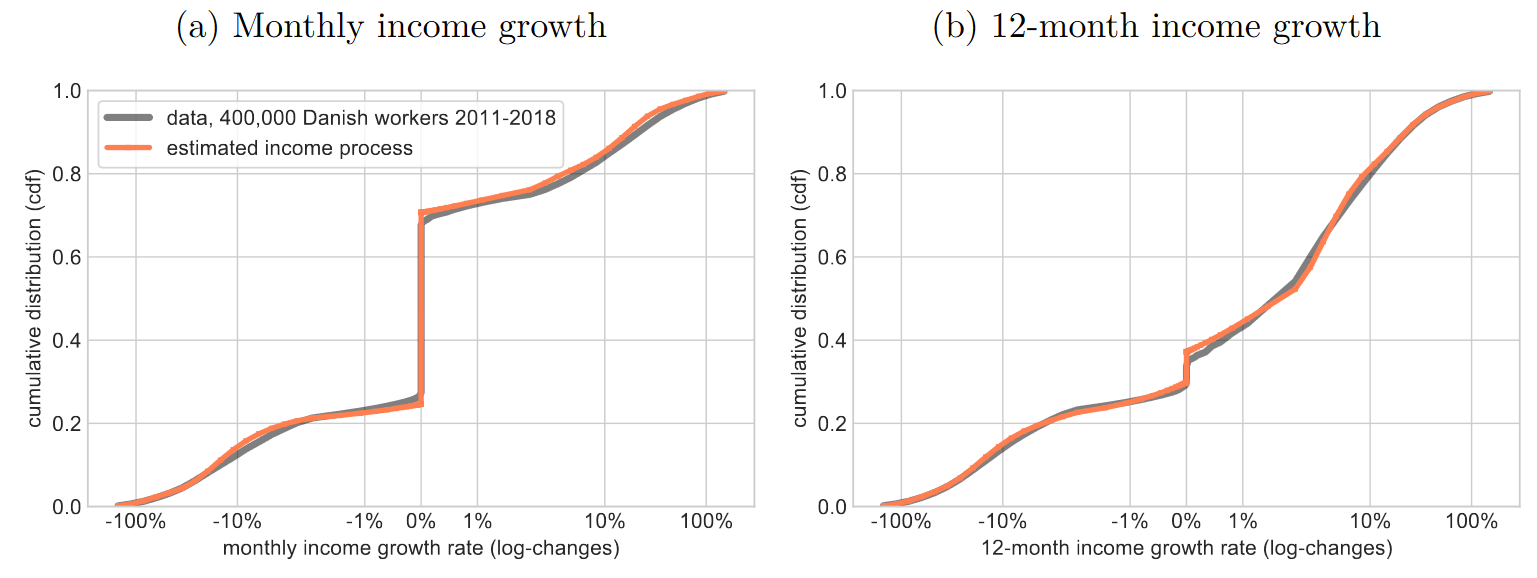
\includegraphics[width=1\textwidth]{figs/HighFreqIncDyn}

Source: Druedahl et. al. (2021)
\end{frame}
%
\begin{frame}{3. Epstein-Zin}

\vspace{-6mm}
\begin{eqnarray*}
v_{t}\left(z_{t},m_{t}\right) & = & \max_{c_{t}}\left[\left(1-\beta\right)\cdot c^{1-\sigma}_{t}+\beta\cdot w^{1-\sigma}_{t+1}\right]^{\frac{1}{1-\sigma}}\\
 & \text{s.t.} & \,\,\,w_{t+1}\equiv\mathbb{E}_{t}\left[v_{t+1}\left(z_{t+1},m_{t+1}\right)^{1-\rho}\right]^{\frac{1}{1-\rho}}\\
 &  & \,\,\,m_{t+1}=(1+r)(m_{t}-c_{t})+y_{t+1}
\end{eqnarray*}

\begin{itemize}
\item \vspace{-4mm}\textbf{Preferences:} 
\begin{enumerate}
\item Patience: $\beta$
\item Intertemporal substitution: $\sigma$
\item Risk-aversion: $\rho$
\end{enumerate}
\item \textbf{Euler-equation:} $c^{-\sigma}_{t}=\beta R\cdot\mathbb{E}_{t}\left[c^{-\sigma}_{t+1}\cdot\left(\frac{w_{t+1}}{v_{t+1}}\right)^{\rho-\sigma}\right]$\vspace{2mm}
\begin{enumerate}
\item FOC: $0=v^{\sigma}_{t}\cdot\left[\left(1-\beta\right)\cdot c^{-\sigma}_{t}-\beta R\cdot w^{\rho-\sigma}_{t+1}\cdot\mathbb{E}_{t}\left[v^{-\rho}_{t+1}\cdot\frac{\partial v_{t+1}}{\partial m_{t+1}}\right]\right]$\vspace{1mm}
\item Envelope condition: $\frac{\partial v_{t}\left(z_{t},m_{t}\right)}{\partial m_{t}}=v^{\sigma}_{t}\cdot\left(1-\beta\right)\cdot c^{-\sigma}_{t}$
\end{enumerate}
\end{itemize}
\end{frame}
%
\begin{frame}{4. Deep learning}
\begin{itemize}
\item \textbf{Curse of dimensionality: }
\begin{enumerate}
\item Many states
\item Many choices
\item Many shocks
\end{enumerate}
\item \textbf{Deep (reinforcement) learning:}
\begin{enumerate}
\item Approximate value and policy functions with \emph{neural networks}
\item Approximate on simulation sample rather than on grid
\item Automatic differentiation (backpropagation) and GPUs for speed
\end{enumerate}
\item \textbf{Examples:} Maliar and Maliar (2021) and Azinovic and Scheidegger
(2022)
\item \textbf{Working paper:} Druedahl and Røpke (2025)

Python package: \color{DarkRed}{\href{https://github.com/NumEconCopenhagen/EconDLSolvers}{EconDLSolvers}}
\end{itemize}
\end{frame}
%

\section{Summary}
\begin{frame}{Summary and what's next}
\begin{itemize}
\item \textbf{This lecture:}
\begin{enumerate}
\item Consumption-saving models (precautionary-saving, buffer-stock target,
intertemporal MPCs)
\item Basic numerical dynamic programming (discretization, numerical integration,
interpolation, VFI)
\item EGM (time iteration, invert Euler-equation)
\item Simulation (monte carlo, histogram)
\end{enumerate}
\item \textbf{Next: }\emph{Stationary equilibrium}
\item \textbf{You should:}
\begin{enumerate}
\item Study the code from this lecture
\item Glance at Aiyagari (1994), \\
>>Uninsured Idiosyncratic Risk and Aggregate Saving<<
\end{enumerate}
\end{itemize}
\end{frame}
%

\end{document}
